
\documentclass[journal,UTF8]{IEEEtran}
%\usepackage{ctex}
\usepackage{color}

%
\usepackage{cite}

\ifCLASSINFOpdf
 \usepackage[pdftex]{graphicx}
  % declare the path(s) where your graphic files are
 \graphicspath{{../pdf/}{../jpeg/}}
  % and their extensions so you won't have to specify these with
  % every instance of \includegraphics
\DeclareGraphicsExtensions{.pdf,.jpeg,.png}
\else
  % or other class option (dvipsone, dvipdf, if not using dvips). graphicx
  % will default to the driver specified in the system graphics.cfg if no
  % driver is specified.
\usepackage[dvips]{graphicx}
  % declare the path(s) where your graphic files are
\graphicspath{{../eps/}}
  % and their extensions so you won't have to specify these with
  % every instance of \includegraphics
\DeclareGraphicsExtensions{.eps}
\fi

\usepackage[cmex10]{amsmath}

\usepackage{algorithmic}

\usepackage{array}


\ifCLASSOPTIONcompsoc
  \usepackage[caption=false,font=normalsize,labelfont=sf,textfont=sf]{subfig}
\else
  \usepackage[caption=false,font=footnotesize]{subfig}
\fi

\hyphenation{op-tical net-works semi-conduc-tor}



\begin{document}

\title{A Review of Artificial intelligence approaches to network management}

\maketitle

% As a general rule, do not put math, special symbols or citations
% in the abstract or keywords.
% * <karyns@accdon.com> 2017-12-24T08:35:37.488Z:
% 
% General note: Language was unclear in many areas. I have done my best to guess at your intended meaning. Please carefully review all edits. 
% 
% ^.
\begin{abstract}
.
 

\end{abstract}

% Note that keywords are not normally used for peerreview papers.
\begin{IEEEkeywords}
Review,Artificial intelligence, Network Management
\end{IEEEkeywords}

% For peer review papers, you can put extra information on the cover
% page as needed:
% \ifCLASSOPTIONpeerreview
% \begin{center} \bfseries EDICS Category: 3-BBND \end{center}
% \fi
%
% For peerreview papers, this IEEEtran command inserts a page break and
% creates the second title. It will be ignored for other modes.
\IEEEpeerreviewmaketitle



\section{Introduction}
There are some labs focusing on machine learning, AI (artificial intelligence), self* (self-configuring, self-healing, self-optimizing and self-protecting), cognitive of NM (network management). Table \ref{table:Labs} shows the information of labs working on AI-based NM. To my best knowledge, it is ranked by importance.

\begin{table*}
	\scriptsize \caption{Information of labs working on AI-based NM}
	\label{table:Labs}
	\begin{center}
		\renewcommand{\arraystretch}{1.4}
		\setlength\tabcolsep{3pt}
		\begin{tabular}{|l|c|c|c|c|c|}
			\hline
			Leader&Country&  University & Personal Publications& collected papers  & key words\\
			\hline
			Boutaba &Canada &University of Waterloo&500  & 2      &       \\
			\hline
			Honggang Zhang & China & Zhejiang University&300  & 7  &       \\
            \hline
 			Hanzo Lajos  & UK  & University of Southampton&1400 & 2  &       \\
            \hline  
 			Riihijarvi J, Mahonen P&Germany&RWTH Aachen University&200 & 1& \\
            \hline  
 			P. Venkataram P&India&Indian Institute of Science& & 2& \\
            \hline 
 			Xiangming Wen&China& Beijing University of Posts and Telecommunications && 2  &       \\
            \hline  
 			Qadir J.&Pakistan&National University of Sciences and Technology&&1& \\
            \hline 
 			Sven G. Bilén&USA& Pennsylvania State University&&1& \\
            \hline         
		\end{tabular}
	\end{center}
\end{table*}


Kumar, et al. \cite{Kumar1997Artificial}, in 1997 a very early year, give a overview of the artificial intelligence in NM which is classified into \textbf{fault management, configuration management, accounting management, performance management, security management} but more expert system than AI technologies are discussed. 20 years later, \cite{Ayoubi2018Machine} from University of Waterloo describes the overview of machine learning as the same classifications meanwhile they have explained more machine learning technologies and provided an impressive framework named C-MAPE (Cognitive-Monitor-Analyze-Plan-Execute over a shared Knowledge) in FIG.\ref{fig:CMAPE}. Then, in \cite{Boutaba2018A}, Boutaba, et al. have a much more comprehensive discussion of machine learning on networking which has over 500 citations. It contains 8 directions: \textbf{traffic prediction, traffic classification, traffic routing, congestion control, resource management, fault management, QoS and QoE management, network security}, illustrated in FIG. \ref{fig:MLinN}. 



Li Rongpeng, et al. \cite{Li2017Intelligent} presents the artificial intelligence int context of 5G and have a different view of the classifications which are \textbf{radio resource management, mobility management, management and orchestration, service provisioning management}.

Jiang and Hanzo Lajos in \cite{Jiang2017Machine} also provides a machine learning paradigms in 5G shown in FIG. \ref{fig:MLin5G}. They distinguish the applications as the type of machine learning.

Qi, et al. \cite{Qi2007Artificial} provides us a comprehensive discussion in network management.



\begin{figure}
	\centering
	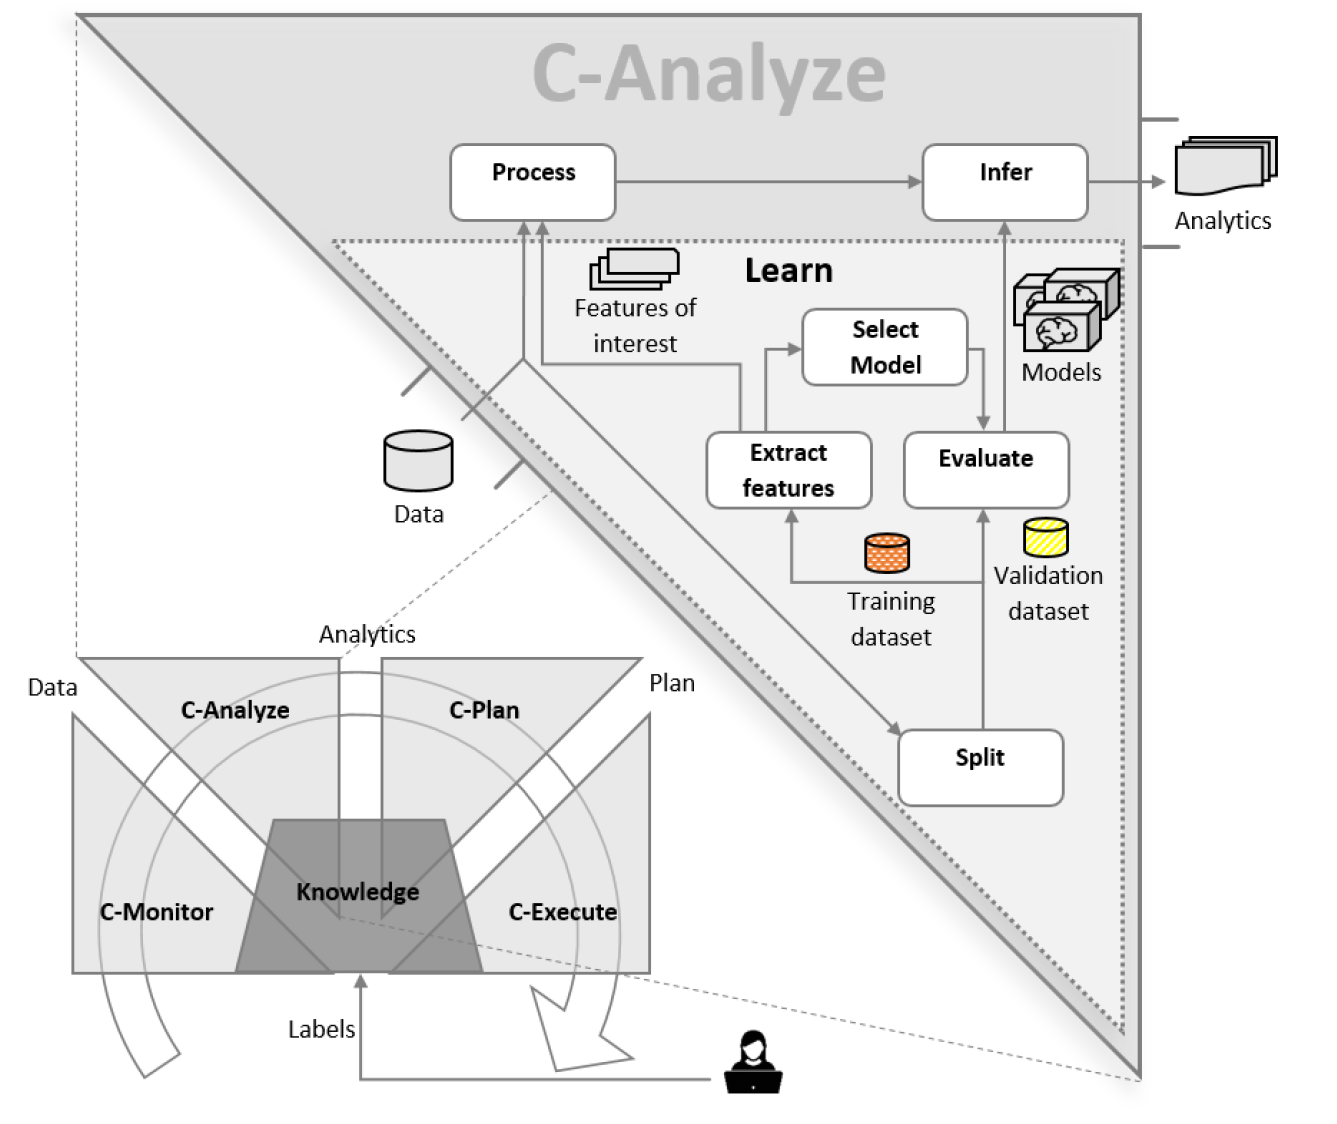
\includegraphics[width=3in]{fig/C-MAPE.png}
	\caption{C-MAPE.}
	\label{fig:CMAPE}
\end{figure}

\begin{figure*}
	\centering
	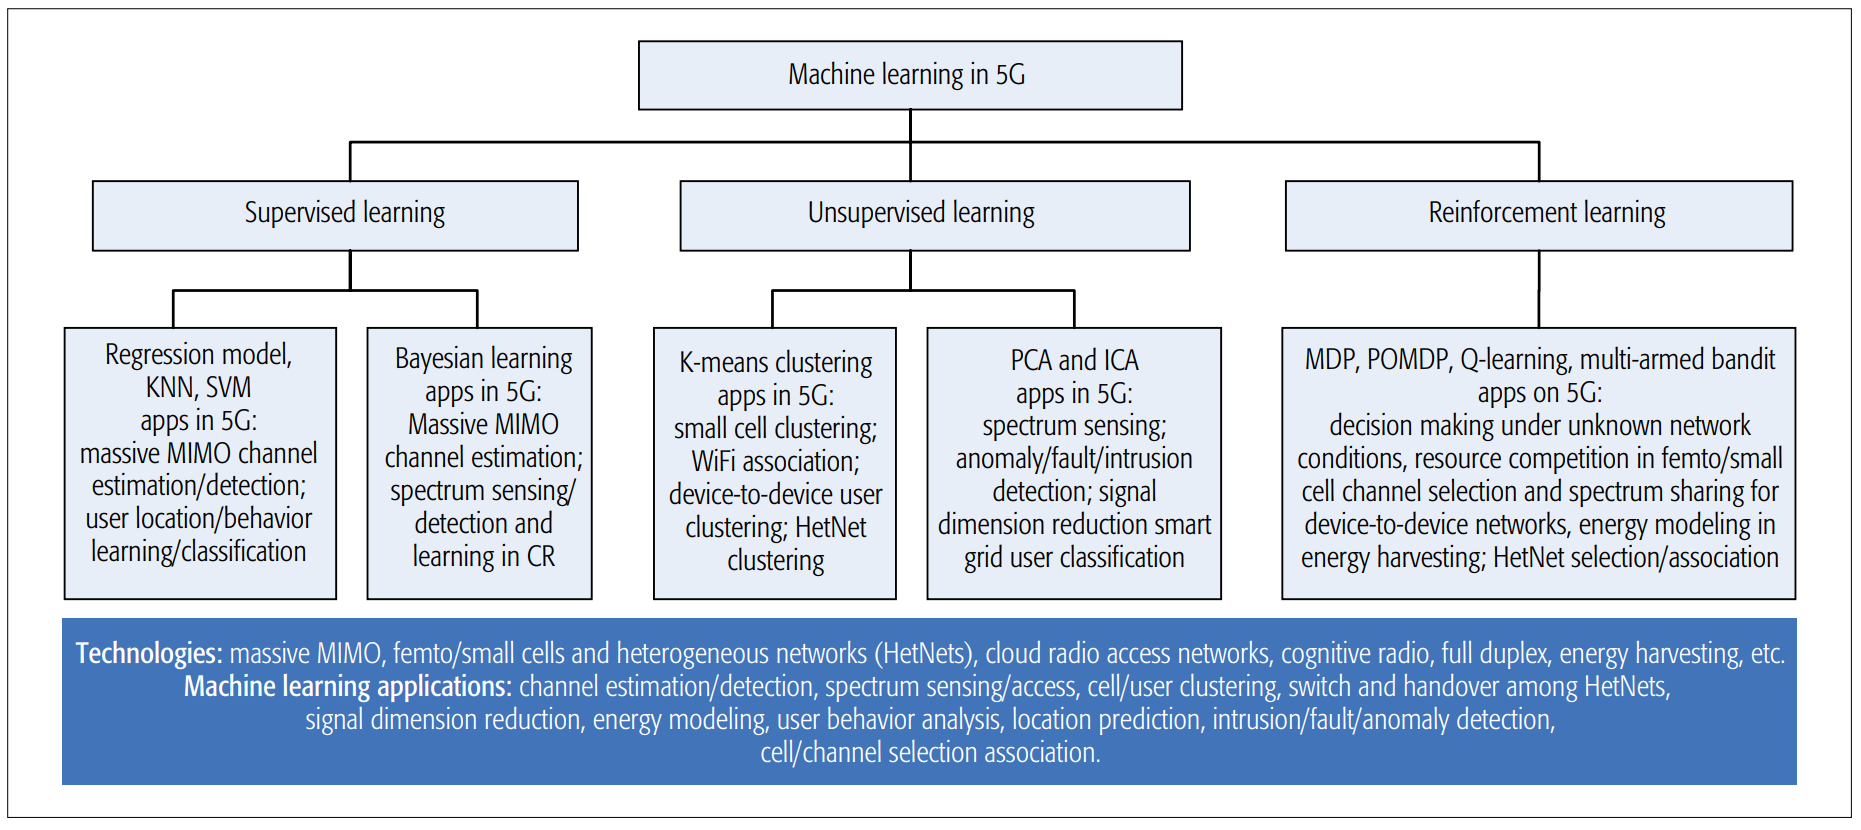
\includegraphics[width=7in]{fig/MLin5G.png}
	\caption{Machine Learning in 5G.}
	\label{fig:MLin5G}
\end{figure*}

 \begin{figure*}
	\centering
	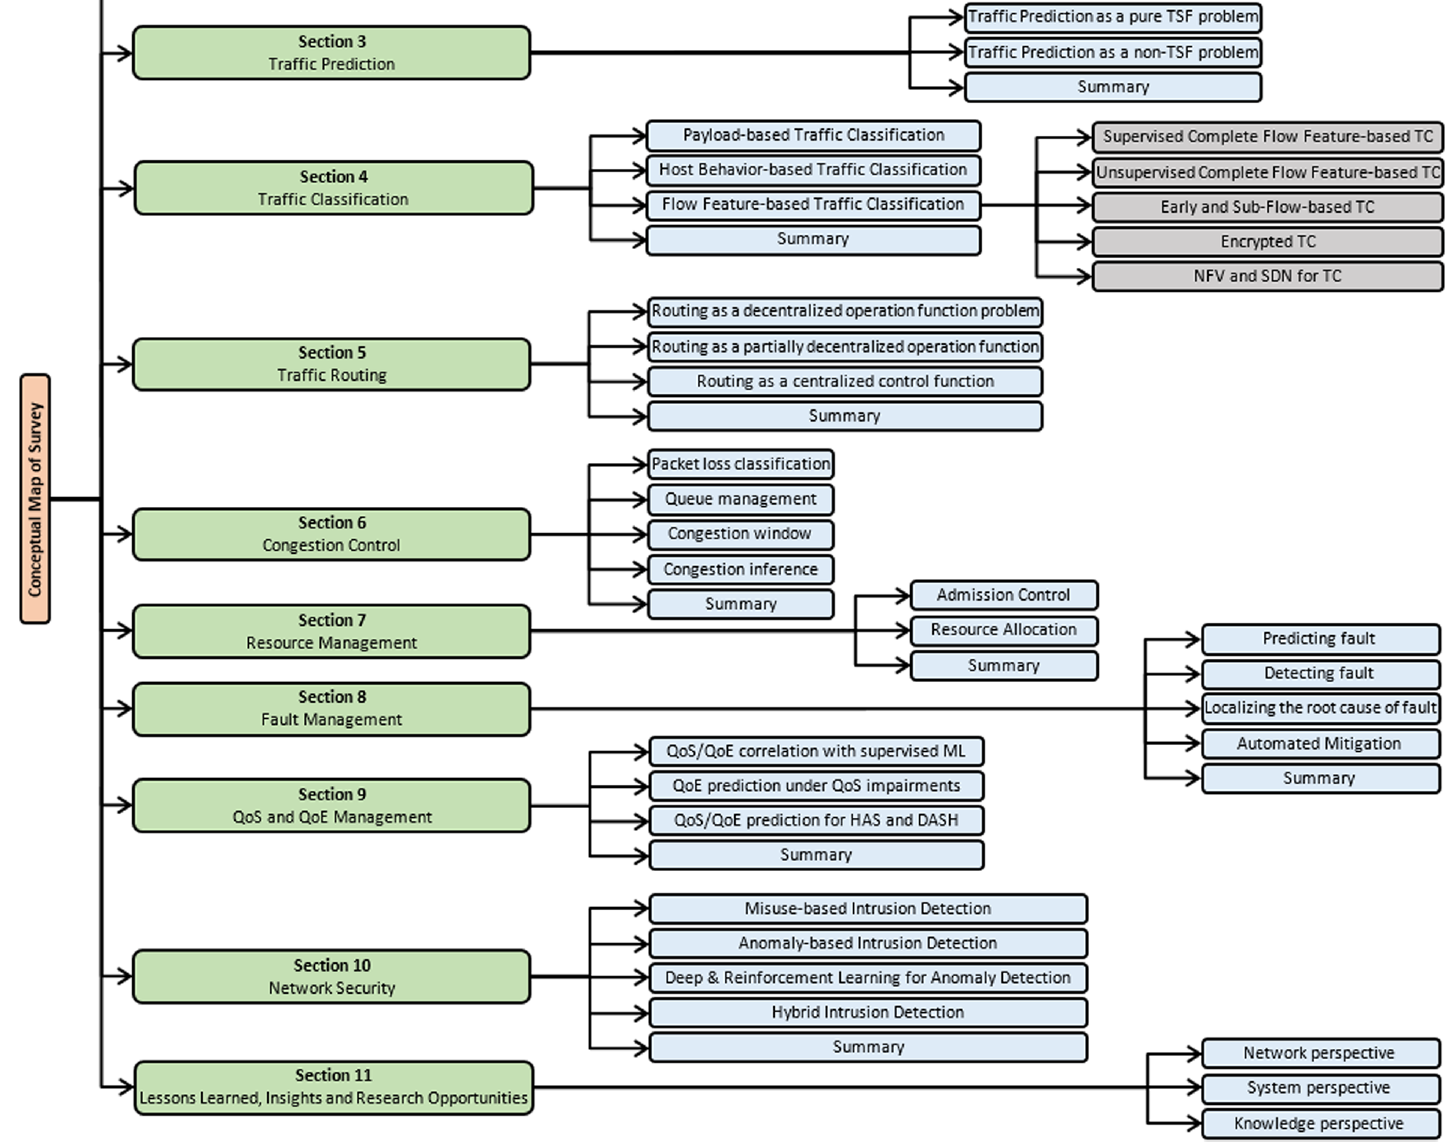
\includegraphics{fig/MLinN.png}
	\caption{Machine Learning in Networking}
	\label{fig:MLinN}
\end{figure*}


\section{Artificial intelligence}
\section{Overview of Network Management}
\subsection{Traffic Classification}
\cite{Williams2006A} is a review of traffic classification. Then a lot of papers\cite{Jin2012A,Huang2012On,Soysal2010Machine} discuss about it.
\subsection{Traffic Prediction}
\cite{Hua2017Traffic} from Zhejiang University is about traffic prediction.
\subsection{Traffic Routing}
Qadir\cite{Qadir2016Artificial} from Pakistan gaves us a review about congnitive routing.
\cite{Hui2002Reinforcement}

\cite{Saleem2017Clustering}

\subsection{Mobility Management}
\cite{Cao2017AIF} poses a AI framework for wireless network management which is used in a case of mobility management, where a ping-pong problem is addressed.  


\subsection{Service Management}
\cite{Rovcanin2015Experimental} uses a reinforcement learning approach to optimize service.

\cite{Zhao2018Deep,Xianfu2018Multi} presents reinforcement approachs to service slicing. 


\subsection{Fault Management}

\cite{Rafique2018Cognitive}


\subsection{Security Management}

\cite{Zheng2016Cognitive,J2018AI}

\subsection{Source management}
\cite{Morozs2016Cognitive,L2017Primary} are about spectrum management.


\subsection{Performance management}
\cite{Kumar2002Network} used the RL to turning the management when performance degradation occurs. From my point of view, it have used the DQL (Deep Q-learning).


\subsection{Platform}
\cite{Ren2018Low}


\section{Opportunities and Challenges}



\section{Conclusion}
\label{conclusion}




\ifCLASSOPTIONcaptionsoff
  \newpage
\fi



% trigger a \newpage just before the given reference
% number - used to balance the columns on the last page
% adjust value as needed - may need to be readjusted if
% the document is modified later
%\IEEEtriggeratref{8}
% The "triggered" command can be changed if desired:
%\IEEEtriggercmd{\enlargethispage{-5in}}

% references section

% can use a bibliography generated by BibTeX as a .bbl file
% BibTeX documentation can be easily obtained at:
% http://www.ctan.org/tex-archive/biblio/bibtex/contrib/doc/
% The IEEEtran BibTeX style support page is at:
% http://www.michaelshell.org/tex/ieeetran/bibtex/
%\bibliographystyle{IEEEtran}
% argument is your BibTeX string definitions and bibliography database(s)
%\bibliography{IEEEabrv,../bib/paper}
%
% <OR> manually copy in the resultant .bbl file
% set second argument of \begin to the number of references
% (used to reserve space for the reference number labels box)

\bibliographystyle{IEEEtran}
\bibliography{reference}

% biography section
%
% If you have an EPS/PDF photo (graphicx package needed) extra braces are
% needed around the contents of the optional argument to biography to prevent
% the LaTeX parser from getting confused when it sees the complicated
% \includegraphics command within an optional argument. (You could create
% your own custom macro containing the \includegraphics command to make things
% simpler here.)
%\begin{IEEEbiography}[{\includegraphics[width=1in,height=1.25in,clip,keepaspectratio]{mshell}}]{Michael Shell}
% or if you just want to reserve a space for a photo:

%\begin{IEEEbiography}[{\includegraphics[width=1in,height=1.25in,clip,keepaspectratio]{fig/Author_HuifengWu.eps}}]{Huifeng Wu} received the Ph.D. degree in computer science and technology from Zhejiang university, Hangzhou, China, in 2006. He is currently a professor in the institute of intelligent and software Technology, Hangzhou Dianzi University. His research interests include software development methods and tools, software architecture, embedded system, intelligent control \& automation.
%	
%\end{IEEEbiography}
%\begin{IEEEbiography}[{\includegraphics[width=1in,height=1.25in,clip,keepaspectratio]{fig/Author_YiYan.eps}}]{Yi Yan} received B.S. in automatic control engineering form Zhejiang Sci-Tech University in 1984, M.S. in computer engineering from Beijing University of Postal Telecommunications in 1990. Currently he is the director and full professor in institute of intelligent and software Technology, Hangzhou Dianzi University. His research interests include embedded system, advanced manufacturing system, intelligent control \& automation, and intelligent instruments.
%	
%	
%\end{IEEEbiography}
%\begin{IEEEbiography}[{\includegraphics[width=1in,height=1.25in,clip,keepaspectratio]{fig/Author_DanfengSun.eps}}]{Danfeng Sun} received M.S. in computer architecture from Hangzhou DianZi University in 2011. He is currently a research assistant in the Institute of Industrial Internet, Hangzhou DianZi University. His research interests include embeded system, motion control and IIoT.
%\end{IEEEbiography}
%\begin{IEEEbiography}[{\includegraphics[width=1in,height=1.25in,keepaspectratio,angle=-90]{fig/Author_ReneSimon.eps}}]{Rene Simon} obtained a doctor of engineering at the Otto-von-Guericke University Magdeburg in 2001. He is Professor of Control Systems at the Department of Automation and Computer Sciences, Harz University of Applied Sciences, Wernigerode, Germany. His major research fields include engineering of automation systems, especially industrial controllers. He is chairman of PLCopen and project leader IEC 61131-10 Ed. 1.0.
%\end{IEEEbiography}



% insert where needed to balance the two columns on the last page with
% biographies
%\newpage


% You can push biographies down or up by placing
% a \vfill before or after them. The appropriate
% use of \vfill depends on what kind of text is
% on the last page and whether or not the columns
% are being equalized.

%\vfill

% Can be used to pull up biographies so that the bottom of the last one
% is flush with the other column.
%\enlargethispage{-5in}



% that's all folks
\end{document}


